% !TEX encoding = UTF-8
% !TEX TS-program = pdflatex
% !TEX root = ../arsclassica.tex
% !TEX spellcheck = it-IT

%************************************************
\chapter{Guide all'uso}
\label{cap:guide}
%************************************************
Lo scopo di questa appendice è formulare delle guide all'utilizzo del software sviluppato a sostengo del lavoro di tesi.

Questa appendice è quindi suddivisa in due sezioni tematiche, una relativa all'utilizzo delle funzionalità offerte dal \pacchettor{} e una relativa all'utilizzo di \acsfont{Sensors} \acs{DLL} per la generazione di dataset da modelli \acs{TSIS}.

\section{Utilizzo del pacchetto RCTBN}\label{sec:package-howto}
Nelle seguenti sottosezioni si illustrano le funzionalità principali offerte da \rctbn{}. Lo scopo è quello di guidare l'utente all'utilizzo del framework delle \acs{CTBN} tramite il succitato pacchetto \lstinline[]|R|.

Prima di addentrarci nella guida all'utilizzo del \pacchettor{} è necessario verificare che il sistema disponga dell'adeguato ambiente \lstinline[]|R| (versione $\ge 3.0$). Inoltre è necessario che il pacchetto \lstinline[]|devtools|\footnote{Il pacchetto \lstinline[]|devtools| è un insieme di funzioni e strumenti finalizzati all'espletamento di processi comuni e fondamentali per lo sviluppo in \lstinline[]|R|. Il codice sorgente di tale pacchetto è disponibile all'indirizzo: \url{https://github.com/hadley/devtools}.} sia correttamente installato. In caso contrario è possibile installare l'ultima versione stabile digitando il seguente comando in una nuova sessione \lstinline[]|R|.

\vspace*{8pt}\inputsourcecode[caption={[Installazione del pacchetto \lstinline$devtools$]Installazione del pacchetto \lstinline$devtools$.},language=R,numbers=none]{codes/devtoolsinstallation}

\subsection{Caricamento del dataset}

\subsection{Calcolo delle sufficient statistics}

\subsection{Calcolo dei parametri}

\subsection{Calcolo delle CIM}

\subsection{Apprendimento}

\subsection{Classificazione}

\subsection{Apprendimento strutturale}

\subsection{Cross-validazione}

\section{Generazione di dataset}\label{sec:create-dataset-howto}
In questa sezione si illustra il processo di generazione di un dataset per le \acs{CTBN} a partire da un modello di traffico \acs{TSIS}, utilizzando l'\acl{RTE} sviluppata in questo lavoro di tesi, \acsfont{Sensors} \acs{DLL}.

\subsection{Sensors DLL}
Al fine di generare un dataset per le \acs{CTBN} che rappresenti l'\keyword{onda quadra} dei sensori a spira magnetica posti su una rete stradale \acs{TSIS} è necessario installare \acsfont{Sensors} \acs{DLL} in \acs{TShell}. Il processo di installazione, come già ampiamente specificato, consiste nel collegamento delle funzioni della succitata \acs{RTE} ai punti di chiamata predefiniti del modulo \acs{CORSIM}. L'intero processo di installazione, propedeutico alla generazione dei dataset, è stato illustrato nella \autoref{subsec:rte-corsim-linking} \vpageref{subsec:rte-corsim-linking}.

Si mostra il processo di generazione del \ds{2} (\vref{sec:dataset-2}).

Come primo passo è chiaramente necessario aprire \acs{TShell} e caricare il modello di traffico per i giorni lavorativi relativo a \emph{Viale Cesare Battisti}. Di seguito si elencano quindi i passi necessari alla generazione del \ds{2}:
\begin{itemize}
	\item nella barra degli strumenti di \acs{TShell} si clicchi l'icona relativa a \acsfont{Sensors} \acs{DLL}
	\item si clicchi sul pulsante relativo alle \emph{\virgolette{proprietà d'esecuzione}} $\vcenter{\hbox{
\includegraphics[scale=.9]{run-props}}}$ e successivamente sulla scheda \emph{\virgolette{proprietà d'esecuzione multipla}}
	\item si selezioni il file \acs{RNS} fornito in allegato a questo lavoro di tesi (e riportato nel sorgente \ref{lst:model2-week-rns} \vpageref{lst:model2-week-rns})\par
	\begin{minipage}{\linewidth}
		\centering
		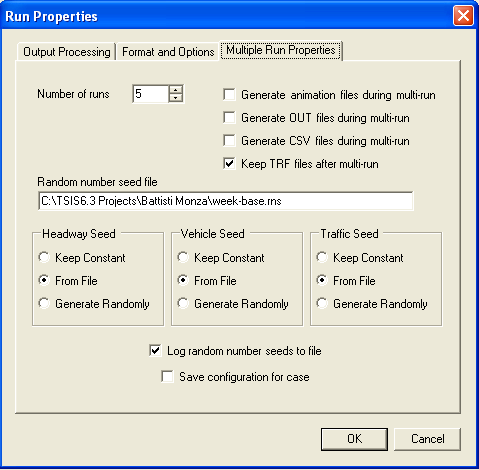
\includegraphics[width=1\linewidth]{multi-run-properties-tsis-next}\captionof{figure}[Esecuzione multipla guidata da file \acs{RNS}]{Selezione del file \acs{RNS} per l'impostazione dell'esecuzione multipla.}\label{fig:multi-run-properties-tsis-next}
	\end{minipage}
	\item si esegua la simulazione cliccando sull'apposito pulsante
	\item conclusa la simulazione, \acsfont{Sensors} \acs{DLL} salva, nella cartella dove il file \acs{TRF} simulato risiede, i file \acs{CSV} di output (riguardo il cui formato si è discusso nella \autoref{subsec:sensors-dll-output}~\vpageref{subsec:sensors-dll-output}).
\end{itemize}

Si osservi che per ogni esecuzione della simulazione viene generato il relativo file di output. Il nome di tali file \acs{CSV} è una concatenazione delle seguenti informazioni: nome del file \acs{TRF} (seguito dal numero dell'esecuzione in caso di esecuzione multipla), data e ora dell'esecuzione, suffisso \lstinline[]|sensors|.

\subsection{Applicativi di supporto}
Ottenuti i file di output di \acsfont{Sensors} \acs{DLL} è necessario trasformarli in un dataset utile al framework delle \acs{CTBN}. A tale scopo sono stati sviluppati degli applicativi, brevemente discussi nella \vref{sec:dataset-tools}.

Il primo passo necessario consiste nella sostituzione dei \emph{\keyword{time period}} con le rispettive classi (si veda a tal riguardo la \vref{tab:ds-2-tp-labels}). A tale scopo è stato sviluppato un programma \lstinline[]|bash| chiamato \lstinline[]|sensors2dataset|.

Riguardo al modello in questione è quindi necessario eseguire il succitato programma nel seguente modo, ripetendo tale passo per tutti i $5$ file di output generati (si ricorda che il modello per i giorni lavorativi viene eseguito infatti $5$ volte, una per ogni giorno lavorativo):

\vspace*{8pt}\inputsourcecode[caption={[Sostituzione dei \emph{time period} con le relative classi]Esecuzione del programma \lstinline[]|bash| per la sostituzione dei \emph{\keyword{time period}} con le relative classi nel file \acs{CSV} relativo al \ds{2}.},language=sh,basicstyle=\footnotesize\ttfamily,numbers=none,label=lst:sensors2dataset]{codes/sensors2dataset2}
Di seguito si spiegano brevemente le opzioni utilizzate:
\begin{itemize}
	\item l'opzione \lstinline[]|i| serve a specificare il percorso del file di input, cioè del file \acs{CSV} generato da \acsfont{Sensors} \acs{DLL}
	\item l'opzione \lstinline[]|t| comunica al programma che il file di input è dotato di intestazione
	\item l'opzione \lstinline[]|r| comunica al programma di rimuovere la colonna relativa ai \emph{\keyword{time period}}
	\item l'opzione \lstinline[]|b| serve a definire i \emph{\keyword{time period}} a partire dai quali una nuova classe deve essere creata e associata
	\item l'opzione \lstinline[]|v| serve per eseguire il programma in modo verboso.
\end{itemize}
Si osservi tuttavia che \lstinline[]|sensors2dataset| implementa molte altre opzioni la cui descrizione è stata tuttavia tralasciata.

Infine, si noti che \lstinline[]|sensors2dataset| non sovrascrive il file di input. Infatti, esso genera automaticamente un nuovo file con le modifiche apportate, concatenando al nome del file di input il suffisso \lstinline[]|dataset|.

A questo punto è possibile scegliere una granularità temporale qualsiasi con cui tagliare il file \acs{CSV}, tenendo presente che \acsfont{Sensors} \acs{DLL} utilizza per il monitoraggio del passaggio dei veicoli sui sensori la massima granularità temporale ottenibile da \acs{CORSIM}, cioè $0.1$ secondi.

Di conseguenza, ipotizzando di voler tagliare il corrente file \acs{CSV} in più file da $100$ secondi, si utilizza il programma \lstinline[]|bash| appositamente sviluppato a tale fine, \lstinline[]|splitfile|.
\vspace*{8pt}\inputsourcecode[caption={[Generazione del \ds{2}]Esecuzione del programma \lstinline[]|bash| finalizzato alla generazione del \ds{2}. Il file di input viene tagliato in più file, ognuno dei quali rappresentante un intervallo temporale di $100$ secondi.},language=sh,numbers=none,basicstyle=\small\ttfamily]{codes/splitfile2}
L'opzione \lstinline[]|n| serve a specificare il numero di righe da cui ogni file deve essere composto. In questo caso quindi, poiché ogni riga rappresenta un intervallo temporale di $0.1$ secondi e desideriamo ottenere dei file che rappresentino intervalli temporali minori o uguali di $100$ secondi, impostiamo il suo valore pari a $1000$.

Si osservi che \lstinline[]|splitfile| salva i file generati in una nuova cartella la cui posizione corrisponde a quella del file di input.

Infine, è possibile ottimizzare il dataset appena generato rimuovendole righe che corrispondono a intervalli temporali durante i quali non è avvenuta alcuna transizione di stato per nessun sensore. A tale scopo viene fornito un programma sviluppato in linguaggio \lstinline[]|R| con interfaccia \lstinline[]|bash| chiamato \lstinline[]|killconsdup|. Esso permette l'ottimizzazione di un singole file \acs{CSV} secondo la logica descritta oppure l'ottimizzazione di tutti i file \acs{CSV} presenti nella cartella di input fornita. Di seguito si illustra la seconda tipologia d'utilizzo di \lstinline[]|killconsdup|.
\vspace*{8pt}\inputsourcecode[caption={[Ottimizzazione del \ds{2}]Esecuzione del programma \lstinline[]|bash| finalizzato alla rimozione delle osservazioni duplicate, cioè delle righe relative agli intervalli temporali durante i quali tutti i sensori sono rimasti nel loro precedente stato.},language=sh,numbers=none]{codes/killconsdup2}
